% 图:BPFGym 闭环,保留原大框套小框结构。上排两个大框(Apps+Workloads、LLM agent,同尺寸),
% 中层 framework 大框含三个后端小框,下层执行环境大框含三个平台小框,层框同尺寸、小框同尺寸、间距统一。
% agent 右缘伸出层框之外,feedback 回路沿右侧单圆角返回,无多重折线。
% 自带库声明与缩放,保证不依赖主文件导言区也能编译且不溢出栏宽。
\usetikzlibrary{arrows.meta,positioning,calc}
\resizebox{\columnwidth}{!}{%
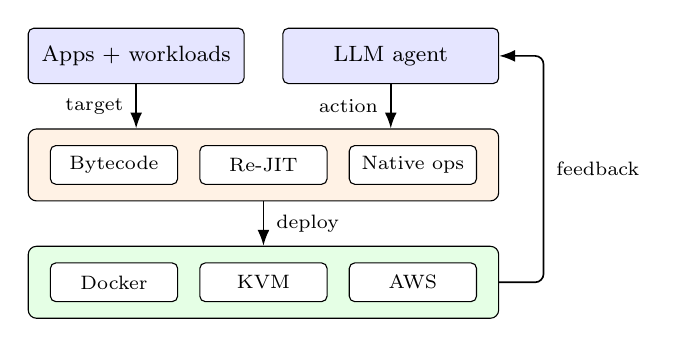
\begin{tikzpicture}[
  bigbox/.style={draw, rounded corners=2pt, font=\footnotesize, minimum width=78pt, minimum height=20pt, inner sep=2pt},
  layer/.style={draw, rounded corners=3pt, minimum width=170pt, minimum height=26pt},
  small/.style={draw, rounded corners=2pt, font=\scriptsize, minimum width=46pt, minimum height=14pt, inner sep=1pt, fill=white},
  lbl/.style={font=\scriptsize},
  arrow/.style={-Latex, semithick, rounded corners=3pt}
]
% 中层与下层:两个同尺寸大层框,各含三个同尺寸小框,水平间距统一 8pt
\node[layer, fill=orange!10] (fw) {};
\node[small] at ($(fw.center)+(-54pt,0)$) (b1) {Bytecode};
\node[small] at (fw.center) (b2) {Re-JIT};
\node[small] at ($(fw.center)+(54pt,0)$) (b3) {Native ops};
\node[layer, fill=green!10, below=16pt of fw] (ex) {};
\node[small] at ($(ex.center)+(-54pt,0)$) (e1) {Docker};
\node[small] at (ex.center) (e2) {KVM};
\node[small] at ($(ex.center)+(54pt,0)$) (e3) {AWS};
% 上排:两个同尺寸大框,与层框边缘取齐,apps 左对左,agent 右对右
\node[bigbox, fill=blue!10, anchor=south west] (apps) at ($(fw.north west)+(0,16pt)$) {Apps + workloads};
\node[bigbox, fill=blue!10, anchor=south east] (agent) at ($(fw.north east)+(0,16pt)$) {LLM agent};
% 箭头:三条垂直直线;feedback 沿右侧通道返回,进 agent 右边,固定边距,双圆角对称
\draw[arrow] (apps.south) -- node[lbl, left=1pt]{target} (apps.south |- fw.north);
\draw[arrow] (agent.south) -- node[lbl, left=1pt]{action} (agent.south |- fw.north);
\draw[arrow] (fw.south) -- node[lbl, right=1pt]{deploy} (ex.north);
\draw[arrow] (ex.east) -- ([xshift=16pt]ex.east) -- node[lbl, right=1pt]{feedback} ([xshift=16pt]ex.east |- agent.east) -- (agent.east);
\end{tikzpicture}%
}
